\section{Problem Formulation and Theoretical Analysis}
\label{sec:analysis}
% 本章分析有限示范下双臂暴露与执行任务的改进条件。
This section studies conditions for improving bimanual exposure and execution from limited demonstrations.
% 暴露动作改变后续操作条件，因此以完整任务后果分析双臂动作偏差。
Because interactions with an occluder change the conditions for subsequent execution, we relate deviations in coordinated actions to failure of the complete task.
% 先由动作误差得到任务界，再说明表示覆盖本身不足以控制该界。
We first derive a task-failure bound under coverage and action-sensitivity conditions, then show why improved representation-level coverage alone is insufficient.
% 再分析可见性与空间关系何时保留专家选择依据，并通过动作重构约束误差迁移。
We next examine when visibility and spatial relationships preserve information needed for expert choices, linking their estimation accuracy to expert-action reconstruction and conditional error transfer.
\subsection{Bimanual Exposure and Execution}
\label{sec:task}

We study bimanual exposure and execution under deformable occlusion.
The arms first establish visibility and access to an occluded target, then complete a prescribed operation and any required restoration.
Because exposure can change both the occluder configuration and target state, subsequent actions must respond to the resulting interaction conditions.
We learn from a finite, fixed demonstration set and evaluate complete-task success within a finite horizon using visual history.

\subsubsection{System, Demonstrations, and Policy}

A single policy coordinates both arms, whose roles may change during execution.
The joint robot-environment state $s_t\in\mathcal S$ includes the arms, target, deformable occluder, and their interaction conditions.
The joint command $u_t\in\mathcal A\subseteq\R^{d_u}$ controls both arms and their end effectors.
The observation $o_t=(I_t^{1:V},\mathbf{x}_t^{\mathrm{prop}})$ contains images from $V\ge1$ cameras and the proprioceptive state $\mathbf{x}_t^{\mathrm{prop}}$.
Over $T$ control steps, the interaction follows
\begin{align}
 s_0&\sim p_0,\nonumber\\
 s_{t+1}&\sim P(\cdot\mid s_t,u_t),\quad 0\le t<T,\nonumber\\
 o_t&\sim O(\cdot\mid s_t),\quad 0\le t\le T.
 \label{eq:interactionmodel}
\end{align}
where $p_0$ is the initial-state distribution and $P$ and $O$ are the transition and observation kernels.
The transition kernel captures coupled arm motion, occluder deformation, and target interaction.

The fixed demonstration set $\mathcal D=\{\zeta_i\}_{i=1}^{N}$ records observations and expert commands for the same task objective:
\begin{equation}
 \zeta_i=(o_0^i,u_0^{\mathrm E,i},o_1^i,\ldots,
 u_{T_i-1}^{\mathrm E,i},o_{T_i}^i).
 \label{eq:demonstrations}
\end{equation}
Here, $T_i$ is the length of trajectory $i$ and the superscript $\mathrm E$ denotes expert commands.
For the analysis, the deployed policy is deterministic and selects $u_t=\pi(\mathcal H_t)$ from the available history $\mathcal H_t$, which contains observations $o_{0:t}$, past commands $u_{0:t-1}$, and any runtime context available before the current decision.

\subsubsection{Learning and Task Objectives}
Let $\pi_{\mathrm E}$ denote the expert policy and let $\nu$ be the population distribution of uniformly sampled demonstration control steps and their histories.
This uses the same control-step weighting as the deployment average introduced below.
The population imitation risk is
\begin{equation}
 R_\nu(\pi)
 :=\E_{(t,h)\sim\nu}\norm{\pi(h)-\pi_{\mathrm E}(h)}^2.
 \label{eq:populationimitationrisk}
\end{equation}
The empirical objective in Section~\ref{sec:method} uses a masked $L_1$ surrogate for this expert-action discrepancy.

The measurable completion function $\Phi:\mathcal S^{T+1}\to\{0,1\}$ evaluates exposure, the prescribed target operation, and any required restoration independently of fixed-time stage boundaries or arm-specific success criteria.
Task-specific criteria are given in Section~\ref{sec:experimentalsetup}.
The completion indicator and success probability are
\begin{equation}
 \Psi=\Phi(s_{0:T}),\qquad
 J(\pi)=\Prob_\pi(\Psi=1).
 \label{eq:visualtask}
\end{equation}
Here, $\Prob_\pi$ is the trajectory law induced by the system and policy.
Learning reduces $R_\nu(\pi)$, whereas deployment seeks to increase $J(\pi)$.
The following analysis states conditions under which these objectives can be related.

\subsubsection{Visual Assessability}
Let $\Omega_{\mathrm{eval}}\subseteq\mathcal S^{T+1}\times\mathcal I^{T+1}$ contain the state and image histories considered under the fixed evaluation setup, where $\mathcal I$ is the space of multi-view images.

\begin{assumption}[Visual assessability]
\label{ass:visualassessability}
There exists a measurable visual decision function $\mathcal V:\mathcal I^{T+1}\to\{0,1\}$
such that, for every $(s_{0:T},I_{0:T}^{1:V})\in\Omega_{\mathrm{eval}}$,
\begin{equation}
 \Phi(s_{0:T})=\mathcal V(I_{0:T}^{1:V}).
 \label{eq:visassumption}
\end{equation}
\end{assumption}
Visual assessability concerns task completion rather than full-state observability.
The evaluation domain includes temporary occlusion but excludes outcomes that remain visually unobservable.
All policy executions and counterfactual comparisons below are restricted to $\Omega_{\mathrm{eval}}$ almost surely.

\subsection{From Imitation Error to Task Performance}
\label{sec:actionanalysis}
An action deviation during exposure can leave the target inaccessible or displace it before execution.
We first relate coordinated action error to complete-task failure, then transfer imitation risk from demonstrations to deployment through a learned representation.

\subsubsection{Task-Performance Difference Between Policies}
\label{sec:actionconsequences}
We compare a policy $\pi$ with a reference policy $\pi_0$ using a finite-horizon performance-difference identity~\cite{ross2014aggrevate,cheng2018value}.
At each history, the identity measures the consequence of selecting an alternative action and then following $\pi_0$.
Given a history $\mathcal H_t=h$ and a candidate action
$a\in\mathcal A$, define the action-value function as the
probability of failing the complete exposure-and-execution task ($\Psi=0$):
\begin{equation}
 Q_t^{\pi_0}(h,a)
 :=\Prob^{a,\pi_0}\!\left(\Psi=0\mid\mathcal H_t=h\right).
 \label{eq:historyactionvalue}
\end{equation}
Here, $\Prob^{a,\pi_0}$ takes action $a$ at time $t$ and follows $\pi_0$ afterward, so an exposure action is evaluated through its consequences for the remaining task.

When the current action is also selected by $\pi_0$, this reduces
to the value function of $\pi_0$, $V_t^{\pi_0}(h) :=Q_t^{\pi_0}\bigl(h,\pi_0(h)\bigr).$
The effect of choosing $a$ instead of $\pi_0(h)$ is therefore
measured by
\begin{equation}
 A_t^{\pi_0}(h,a)
 :=Q_t^{\pi_0}(h,a)-V_t^{\pi_0}(h).
 \label{eq:actionconsequence}
\end{equation}
Thus, $A_t^{\pi_0}(h,a)>0$ indicates an increase in failure probability, whereas $A_t^{\pi_0}(h,a)<0$ indicates a decrease.

The comparison requires a common task and environment.
\begin{assumption}[Common task and environment]
\label{ass:commonprocess}
The compared policies share the same initial distribution and
task-completion criterion. Given a history $h$ and an action $a$,
the next available history follows a conditional distribution
that does not otherwise depend on the policy.
The reference policy $\pi_0$ is defined on all histories
involved in the comparison.
\end{assumption} 
% 比较的是同一任务实例分布与相同交互观测机制，而非强制相同后续轨迹。
The policies may induce different trajectories, but the initial task distribution and interaction and sensing mechanisms remain fixed.

Let $F(\pi)=1-J(\pi)$ denote the task-failure probability of policy $\pi$.
To evaluate $\pi$ relative to $\pi_0$, we set $a=\pi(h)$
and aggregate the resulting action consequences along trajectories generated by $\pi$.

Applying the finite-horizon performance-difference identity~\cite{kakade2002,ross2014aggrevate,cheng2018value}
to these one-step action effects gives
\begin{equation}
 F(\pi)-F(\pi_0)
 =\E_\pi\!\left[
 \sum_{t=0}^{T-1}A_t^{\pi_0}(\mathcal H_t,\pi(\mathcal H_t))
 \right].
\label{eq:pd}
\end{equation}
The expectation is over trajectories generated by $\pi$, so the action effects are evaluated at histories visited by the evaluated policy.
Appendix~\ref{app:pdidentity} gives the proof.


\subsubsection{Task-Failure Bounds from Imitation Risk}
\label{sec:actionerrorbound}
Taking the expert policy as the reference,
we show that the imitation risk $R_\nu(\pi)$ bounds task-failure probability $F(\pi)$
when demonstrations sufficiently cover exposure and execution histories encountered at deployment
and action deviations have bounded task consequences.

Imitation risk is evaluated under the demonstration distribution $\nu$,
but deployment histories may follow a different distribution because actions depend on $\pi$.
Let $\mu_\pi^t$ denote the distribution of $(t,\mathcal H_t)$ at control step $t$ under $\pi$.
The distribution $\bar\mu_\pi=T^{-1}\sum_{t=0}^{T-1}\mu_\pi^t$ corresponds to choosing
a control step uniformly and observing its history.

% 对待评价策略，假设部署分布由示范分布以有限常数控制。
\begin{assumption}[Demonstration coverage]
\label{ass:democoverage}

For the evaluated policy $\pi$, there exists a uniform constant
$1\le C<\infty$ such that
\[
\bar\mu_\pi(\mathcal B)\le C\,\nu(\mathcal B)
\]
for every measurable set $\mathcal B$ of pairs $(t,h)$.
\end{assumption}
This excludes deployment histories absent from the demonstration distribution and limits probability underestimation after occluder and target interactions.

\begin{assumption}[Action sensitivity]
\label{ass:actionsensitivity}
Let $A_t^{\mathrm E}$ denote the action effect with the expert
policy as the reference.
For a fixed action scale, there exists a uniform constant
$0\le L<\infty$ such that
\[
|A_t^{\mathrm E}(h,a)|
\le L\norm{a-\pi_{\mathrm E}(h)}
\]
for all relevant $(t,h,a)$.
\end{assumption}
This translates coordinated command error into a change in eventual failure probability.
Deformable interaction does not guarantee such regularity near changes in contact or accessibility.

Following the connection between deployment imitation error
and task cost~\cite{ross2011}, Assumptions~\ref{ass:democoverage}
and~\ref{ass:actionsensitivity}, together with the
performance-difference identity, yield the following bound (Appendix~\ref{app:actionriskbound}):
\begin{equation}
 F(\pi)\le F(\pi_{\mathrm E})+TL\sqrt{C R_\nu(\pi)}.
 \label{eq:successbound}
\end{equation}

Here, $C$ measures demonstration-to-deployment shift and $L$ measures task sensitivity to action deviations.
The bound shows that imitation accuracy controls task failure only under both conditions.

\subsubsection{Imitation-Risk Transfer Through Representations}
\label{sec:representationcoverage}
We next replace complete-history coverage with coverage in a learned representation and account for the error introduced by merging histories.

Assumption~\ref{ass:democoverage} can fail even after an arbitrarily small action deviation.
For $T\ge2$, suppose the expert always executes $u_0=0$, whereas the learned policy executes
an admissible $u_0=\varepsilon\ne0$.
Histories recording $u_0=\varepsilon$ then occur under the learned policy
but have zero probability under the expert demonstration distribution.
No finite coverage constant $C$ can satisfy the assumption.

A representation can merge such distinctions, potentially relaxing coverage requirements,
but may also discard information needed to distinguish action consequences.
For exposure and execution, useful compression should suppress irrelevant appearance variation without merging situations that require further exposure with those that permit target interaction.
This tension between distributional alignment and information loss under a noninvertible representation
also appears in domain-adaptation analyses~\cite{johansson2019support,zhao2019invariant}.

Fix the policy and expert, set $\mu=\bar\mu_\pi$, and let $Z=\phi(t,\mathcal H_t)$ be a measurable causal representation that retains the time index.
Let $\mu_Z$ and $\nu_Z$ be the representation distributions induced by $\mu$ and $\nu$.

\begin{assumption}[Representation coverage]
\label{ass:representationcoverage}
There exists $1\le C_\phi<\infty$ such that
\begin{equation}
 \mu_Z(\mathcal B)\le C_\phi\nu_Z(\mathcal B)
 \label{eq:representationcoverage}
\end{equation}
for every measurable representation event $\mathcal B$.
\end{assumption}

Histories merged at the same representation can still have different action errors.
Define
\begin{align}
 e(h)&=\norm{\pi(h)-\pi_{\mathrm E}(h)},\nonumber\\
 m_\rho(z)&=\E_\rho[e(h)^2\mid Z=z],\quad \rho\in\{\mu,\nu\},\nonumber\\
 D_\phi&=\E_{z\sim\mu_Z}|m_\mu(z)-m_\nu(z)|.
 \label{eq:conditionalerrordiscrepancy}
\end{align}
Assuming square-integrable action error and measurable conditional means, representation coverage gives
\begin{equation}
 \E_{\mu}e(h)^2
 \le C_\phi R_\nu(\pi)+D_\phi.
 \label{eq:representationrisktransfer-main}
\end{equation}
If Assumption~\ref{ass:actionsensitivity} also holds, the performance-difference identity gives
\begin{equation}
 F(\pi)\le F(\pi_{\mathrm E})
       +TL\sqrt{C_\phi R_\nu(\pi)+D_\phi}.
 \label{eq:representationcoveragebound}
\end{equation}

Appendix~\ref{app:representationcoverage} gives the proof.
Equation~\eqref{eq:representationcoveragebound} shows why improved representation coverage alone is insufficient.
A useful representation must reduce $C_\phi$ without increasing the conditional-error discrepancy $D_\phi$ enough to offset that gain.

\subsection{Task-Relevant Information Preservation}
\label{sec:representationanalysis}
We now bound $D_\phi$ by requiring the representation to preserve information from which expert bimanual actions can be reconstructed.

\subsubsection{Semantic Guidance and Decision Representations}
Semantic guidance can encourage an encoder to merge appearance differences while retaining object-level structure relevant to action selection.
However, appending a deterministic semantic map while retaining the original red--green--blue (RGB) input does not itself improve the best coverage constant because the RGB input remains recoverable by projection.
The relevant object is therefore the learned decision representation $Z$, not the number of input modalities.
To control $D_\phi$, this representation must preserve information that supports a common expert-action rule under both demonstration and deployment distributions.
This decision-relevant view is consistent with information-state and behaviorally grounded representation analyses~\cite{subramanian2022ais,zhang2021dbc}.

% \subsubsection{任务信息与专家动作重构}
\subsubsection{Task Information and Expert-Action Reconstruction}
We examine when retained visibility and interaction geometry, together with execution context, suffice to approximate the expert's coordinated actions.
The reconstruction error depends on both what the selected information fails to explain and how accurately it is estimated.

Continue with $\mu=\bar\mu_\pi$ and the demonstration distribution $\nu$.
Write $\pi(h)=p(Z)$ for the same measurable policy readout under both distributions.
We define a task descriptor vector $G\in\R^{d_G}$ to describe the target's exposure and its spatial relationships to the occluder, tools, and goal.
Depending on the prescribed operation, its components can include visible area, separation from the occluder, tool--target displacement, and target--goal proximity.
Semantic masks provide geometric supervision for selected components, rather than a complete description of contact or deformation.
Let $\chi$ denote task-specified proprioceptive and execution context, selected in advance rather than identified with the unrestricted history.
For bimanual coordination, $\chi$ includes both arms' configurations and any available context needed to distinguish exposure, target interaction, and restoration without requiring an explicit phase label.
Assume measurable readouts $r_\chi$ and $r_G$ such that $\chi=r_\chi(Z)$ and $\widehat G=r_G(Z)\in\R^{d_G}$.
For $\rho\in\{\mu,\nu\}$, define $\delta_{G,\rho}=\E_\rho\norm{G-\widehat G}$.
These quantities must be defined under both distributions, with an explicit convention for unavailable components.

% \begin{assumption}[描述量条件下的专家选择]
\begin{assumption}[Descriptor-conditioned expert selection]
\label{ass:expertselection}
There exists a common measurable rule $g_{\mathrm E}$ mapping descriptors and context to $\mathcal A$ such that, for $\rho\in\{\mu,\nu\}$,
\begin{equation}
 \E_\rho\norm{\pi_{\mathrm E}(h)-g_{\mathrm E}(G,\chi)}
 \le\epsilon_{\mathrm{sel},\rho}.
 \label{eq:expertselectionapprox}
\end{equation}
For a finite constant $K_{\mathrm E}\ge0$,
\begin{equation}
 \norm{g_{\mathrm E}(G,\chi)-g_{\mathrm E}(\widehat G,\chi)}
 \le K_{\mathrm E}\norm{G-\widehat G}
 \label{eq:expertselectionsensitivity}
\end{equation}
holds almost surely under both distributions, with finite $\epsilon_{\mathrm{sel},\rho}$ and $\delta_{G,\rho}$.
\end{assumption}
Here, $\epsilon_{\mathrm{sel},\rho}$ measures expert commands unexplained by $(G,\chi)$, including omitted contact or deformation, while $K_{\mathrm E}$ measures sensitivity to descriptor error.
Task relevance alone does not imply this condition: equally successful actions may reflect different expert choices.

Define $\widehat a_{\mathrm E}(Z)=g_{\mathrm E}(\widehat G,\chi)$.
The triangle inequality yields
\begin{equation}
 \E_\rho\norm{\pi_{\mathrm E}(h)-\widehat a_{\mathrm E}(Z)}
 \le b_\rho
 :=\epsilon_{\mathrm{sel},\rho}+K_{\mathrm E}\delta_{G,\rho}.
 \label{eq:expertreconstruction}
\end{equation}
Appendix~\ref{app:expertreconstruction} gives the derivation.
Supervising descriptor readouts targets the estimation term, while the choice of descriptors and context determines how well expert actions can be explained.

% \subsubsection{条件模仿误差差异的约束}
\subsubsection{Bounds on Conditional Imitation-Error Discrepancy}
\label{sec:relationtransfer}
Expert-action reconstruction connects information preservation to the discrepancy in Section~\ref{sec:representationcoverage}.
Because both $\pi(h)=p(Z)$ and $\widehat a_{\mathrm E}(Z)$ depend on the same representation, their squared difference is a common function under $\mu$ and $\nu$.
Expert reconstruction error bounds how far the actual conditional imitation errors depart from this function.

Assume a finite action-set diameter $B_{\mathcal A}=\sup_{a,a'\in\mathcal A}\norm{a-a'}$ under a fixed action scale.
% \begin{proposition}[通过专家动作重构约束条件误差迁移]
\begin{proposition}[Conditional-error transfer through expert reconstruction]
\label{prop:relationtransfer}
Under Assumptions~\ref{ass:representationcoverage} and~\ref{ass:expertselection}, with $b_\rho$ defined in~\eqref{eq:expertreconstruction},
\begin{equation}
 D_\phi\le 2B_{\mathcal A}(b_\mu+C_\phi b_\nu).
 \label{eq:relationdiscrepancybound}
\end{equation}
If Assumption~\ref{ass:actionsensitivity} also holds,
\begin{equation}
 F(\pi)\le F(\pi_{\mathrm E})
 +TL\sqrt{C_\phi R_\nu(\pi)+2B_{\mathcal A}(b_\mu+C_\phi b_\nu)}.
 \label{eq:relationtransferfailure}
\end{equation}
\end{proposition}
The proof is in Appendix~\ref{app:relationtransfer}.
The bound separates the roles of the learning signals and assumptions.
Action imitation targets $R_\nu(\pi)$, representation coverage is summarized by $C_\phi$, descriptor supervision targets $\delta_{G,\rho}$ through $b_\rho$, and $\epsilon_{\mathrm{sel},\rho}$ records task information omitted by the selected descriptors and context.
For a fixed expert baseline, horizon, and action sensitivity, the task-failure bound tightens only when these combined terms decrease.

% 提前提交双栏方法图，使其显示在方法正文附近的前一页。
\begin{figure*}[!t]
\centering
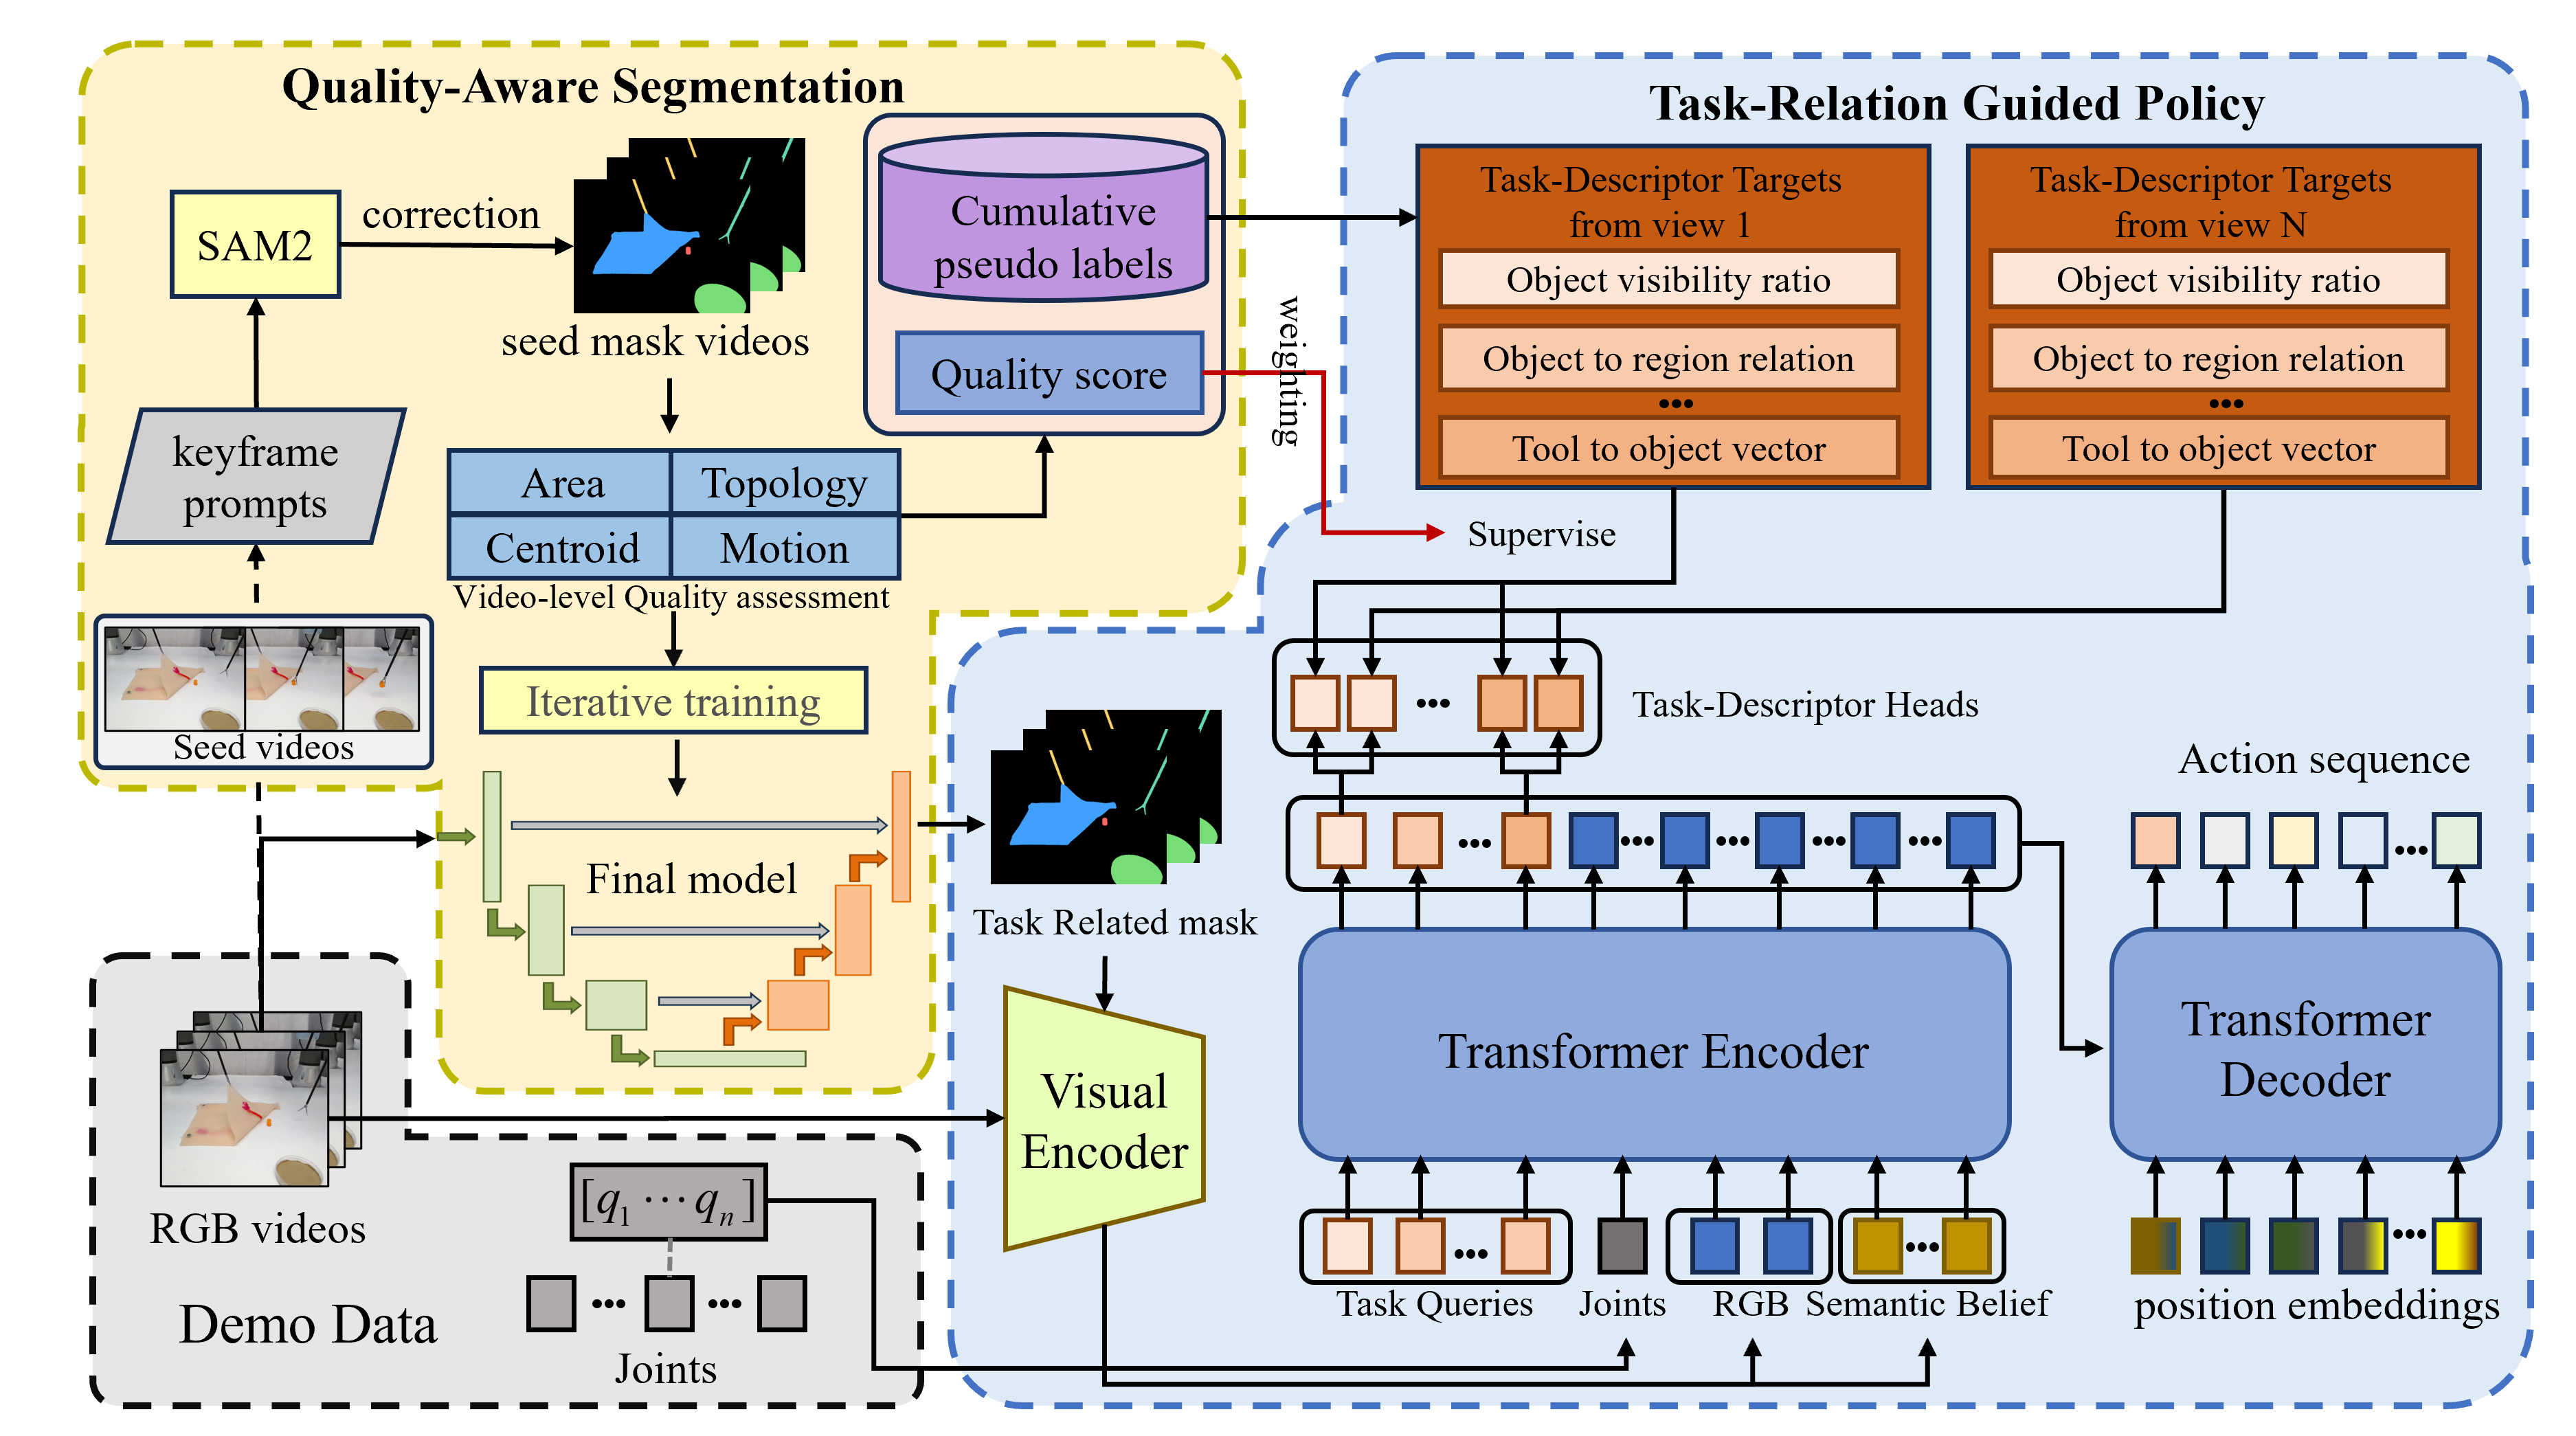
\includegraphics[width=\textwidth]{myfigure/fig1.png}
\caption{Method overview. Quality-aware cumulative annotation provides frozen per-view segmenters, task-descriptor targets, and reliability weights. A shared visual backbone encodes the RGB and semantic streams. One learned query per task relation integrates visual and proprioceptive information, is supervised by independent view-specific heads, and remains available to the action decoder for action-chunk prediction.}
\label{fig:architecture}
\end{figure*}

